\documentclass[british]{extreport}
\usepackage{fourier}
\usepackage[T1]{fontenc}
\usepackage{geometry}
\geometry{verbose,tmargin=2cm,bmargin=2cm,lmargin=2cm,rmargin=2cm}
\setcounter{tocdepth}{3}
\usepackage{babel}
\usepackage{array}
\usepackage{enumitem}
\usepackage[xetex]{graphicx}
\usepackage{setspace}
\usepackage[authoryear]{natbib}
\usepackage{microtype}
\onehalfspacing
\usepackage[unicode=true,pdfusetitle,bookmarks=true,bookmarksnumbered=true,bookmarksopen=false,breaklinks=false,pdfborder={0 0 0},pdfborderstyle={},backref=page,colorlinks=false]
 {hyperref}

\makeatletter

\providecommand{\tabularnewline}{\\}

\newlength{\lyxlabelwidth}

\AtBeginDocument{
  \def\labelitemi{\(\star\)}
}

\makeatother

\begin{document}
\title{\noindent \textbf{LECTURE NOTES\\ON\\COMPUTER ARCHITECTURE\\AND\\ORGANIZATION}}
\author{\noindent AGNI DATTA}

\maketitle
\noindent \tableofcontents{}

\chapter{INTRODUCTION TO SYSTEM ARCHITECTURE AND ORGANISATION}

\pagebreak{}

\section{System Architecture}

\noindent A system architecture is a conceptual model that specifies
the structure, behaviour, and additional perspectives of a system.
An architectural description is a formal description and representation
of a system that is arranged in such a manner that it allows for reasoning
about the system's structures and actions. A system architecture can
be made up of system components and created subsystems that will function
together.

\noindent In summary,
\begin{enumerate}
	\item The architecture of a computer system can be considered as a catalogue
	      of tools or attributes that are visible to the user such as instruction
	      sets, number of bits used for data, addressing techniques, etc.
	\item Controls the logical aspects of a computer system.
	\item The architecture refers to those attributes of the system visible
	      to the programmer.
\end{enumerate}

\section{System Organisation}

\noindent Organization of a computer system defines the way system
is structured so that all those catalogued tools can be used. The
significant components of Computer organization are ALU, CPU, memory
and memory organization.

\noindent In summary,
\begin{enumerate}
	\item Organization of a computer system defines the way system is structured
	      so that all those catalogued tools can be used.
	\item Physical aspects of computer system
	\item Computer organization is used to study the basic computer hardware
	      structure and behaviour of digital computers.
\end{enumerate}

\subsection{Importance of Computer Organization and Architecture}

These are a few important points,
\begin{itemize}
	\item Computer Architecture and Organisation is necessary to understand
	      the designing and functioning of the various components to process
	      information digitally.
	\item Computer Architecture and Organisation study focuses on the interface
	      between hardware and software.
	\item Computer Architecture and Organisation tells the way of operating
	      hardware components and their interconnections in computer.
	\item Computer Architecture and Organisation provides an organized way of
	      working with different hardware components together in one place.
	\item Computer Architecture and Organisation provides detailed knowledge
	      of the system components, Circuit designs, Structure of Instruction,
	      Computer arithmetic, Assembly programming, processor control, logical
	      design, and performance method.
	\item Computer Architecture and Organisation proves that different computer
	      organizations can use the same architecture. For example, Intel and
	      AMD make x86\_64 CPU (processor is of 64 bits), but INTEL makes its
	      organization on x86\_64, and AMD makes its own, which means the processor
	      is 64 bits. Still, internal circuits, working, interconnections will
	      be different.
	\item Computer Architecture and Organisation subject helps the computer
	      engineers to understand the components functioning, working, characteristics,
	      performance, and their interactions.
\end{itemize}

\section{Types of Computers}

A computer is a machine that can be configured to automatically perform
arithmetic or logical functions. Programs are general collections
of operations that modern computers could do. These programmes allow
computers to execute a variety of activities. A computer system is
a \textquotedbl complete\textquotedbl{} computer that comprises the
necessary hardware, operating system (main software), and peripheral
devices for \textquotedbl full\textquotedbl{} functioning. This word
can also apply to a collection of computers that are linked and work
together, such as a computer network or a computer cluster.

\noindent The four basic types of computers are as under:

\subsection{Supercomputers}

\noindent A supercomputer is designed to do activities that require
extensive numerical computations, such as weather forecasting, fluid
dynamics, nuclear simulations, theoretical astrophysics, and complicated
scientific computations. A supercomputer is a computer that is at
the cutting edge of current processing capability, notably computation
speed. The word \textquotedblleft supercomputer\textquotedblright{}
is very flexible, and the speed of today's supercomputers tends to
become representative of tomorrow's average computer. FLOPS, or floating-point
calculations per second, are the units of measurement for supercomputer
processing speeds.

\noindent Calculating complicated mathematical equations in real numbers
is an example of a floating-point procedure. Supercomputers are the
most powerful in terms of computing capabilities, memory capacity
and speed, I/O technology, and topological concerns such as bandwidth
and latency, but they are highly expensive and not cost-effective
for batch or transaction processing. These computers were created
in the 1970s and are the fastest and most powerful computers available.

\subsection{Mainframe Computers}

The term mainframe computer was used to distinguish between the conventional,
big, institutional computer designed to serve numerous users and the
smaller, single-user computers. These computers are capable of handling
and processing massive volumes of data in a short period of time.
Mainframe computers are utilised in big organisations such as the
government, banks, and companies. They are measured in MIPS (million
instructions per second) and can handle hundreds of millions of users
concurrently.

\subsection{Minicomputers}

Minicomputers (abbreviated \textquotedbl minis\textquotedbl ) are
a type of multi-user computer that falls somewhere in the centre of
the computing spectrum, between the smallest mainframe computers and
the largest single-user systems (microcomputers or personal computers).
The name super-mini computer, or simply super-mini, was used to designate
more powerful minicomputers with capabilities comparable to mainframes.
At a period when most minicomputers (such as the PDP-11, Data General
Eclipse, or IBM Series/1) were 16-bit, super-minis (such as the DEC
VAX or Data General Eclipse MV/8000) were 32-bit. These traditional
minicomputers, found throughout small to medium-sized businesses,
laboratories, and embedded in (for example) medical facility CAT scanners
for the last few decades of the 20th century, were mostly rack-mounted
and connected to one or more terminals or tape/card readers, like
mainframes and unlike most personal computers, but mandated less space
and electrical power than a typical mainframe. The term \textquotedbl minicomputer\textquotedbl{}
currently refers to higher-end SPARC, POWER, and Itanium-based systems
from Oracle Corporation, IBM, and Hewlett-Packard, and the size is
now generally smaller, such as a tower case.

\subsection{Microcomputers}

In the late twentieth century, microcomputers became the most popular
form of computer. With the introduction of systems based on single-chip
microprocessors, the term \textquotedbl microcomputer\textquotedbl{}
was coined. The Altair 8800, released in 1975, was one of the most
well-known early system. The word \textquotedbl microcomputer\textquotedbl{}
has almost become obsolete.

\subsection{Comparison of Processors}
\begin{center}
	\begin{tabular}{|>{\raggedright}m{40mm}|>{\raggedright}m{40mm}|>{\raggedright}m{40mm}|>{\raggedright}m{40mm}|}
		\hline
		\textbf{MICRO COMPUTER}                                & \textbf{MINI COMPUTER}                                                    & \textbf{MAINFRAME COMPUTER}                                            & \textbf{SUPER COMPUTER}\tabularnewline
		\hline
		\hline
		A microcomputer is a small relatively inexpensive computer with a
		microprocessor as its central processing unit (CPU).   & It was first developed by IBM in mid 1960. Also called midrange computer. & It is type of computers that generally are known for their large size,
		amount of storage, processing power and high reliability. It first
		appeared in 1940.                                      & It consists of tens of thousands of processor that are able to perform
		billions and trillions of calculations or computations per seconds.\tabularnewline
		\hline
		It includes a microprocessor, memory, and I/O devices. & It may content one or more processors, support multiprocessing and
		tasking and generally resilient to high workloads.     & Used by large organizations for mission-critical applications required
		for high volume data processing. Ability to run multiple operating
		system.                                                & Designed for enterprises and organization which need massive computing
		power.\tabularnewline
		\hline
		Example: IBM PC, Apple Macintoshes, Dell Home PC       & Example: DEC\textquoteright s,VAX, RANGE                                  & Example: IBM zSeries, System z9                                        & Example: IBM Sequoia, PARAM, Fujitsu Fugaku\tabularnewline
		\hline
	\end{tabular}
	\par\end{center}

\chapter{Basic Structure of Computer}

\pagebreak{}

\section{Basic Functional Units}
\begin{center}
	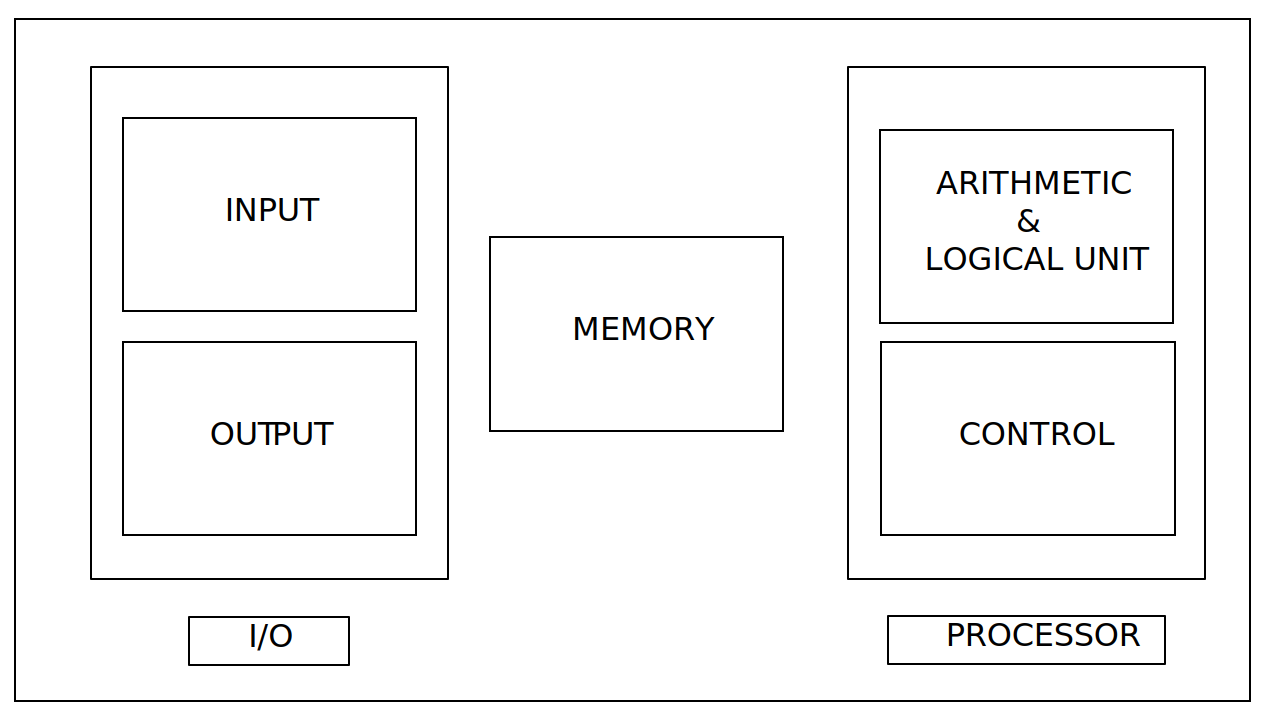
\includegraphics[scale=0.3]{Picture/FUNCTIONAL_UNIT}
	\par\end{center}

\section{Information Handled by Computer}

\subsection{Instructions/Machine Instructions}
\begin{center}
	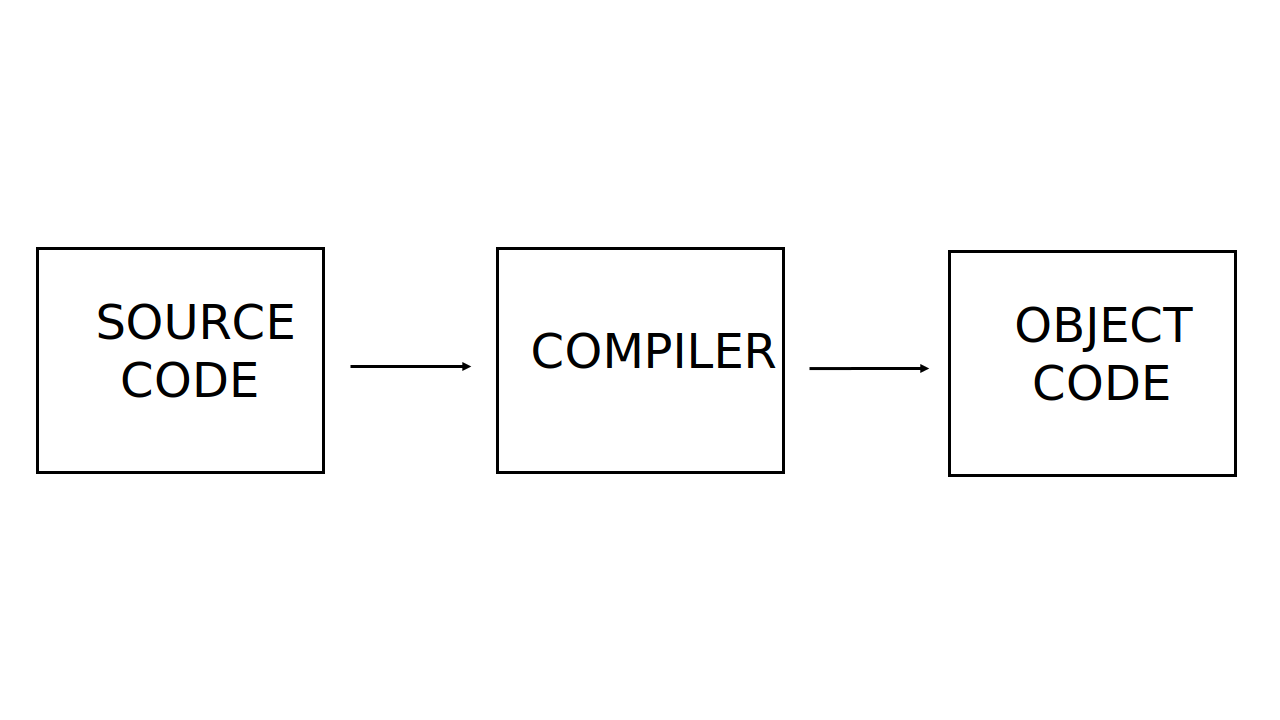
\includegraphics[scale=0.25]{Picture/COMPILER_DIAGRAM}
	\par\end{center}
\begin{itemize}
	\item Govern the transfer of information within a computer as well as between
	      the computer and its I/O devices
	\item Specify the arithmetic and logic operations to be performed
	\item Program is a list of instruction that perform a task
	\item Data used as operands by the instructions source program
	\item Encoded in binary code: 0 and 1
\end{itemize}
\vfill{}


\subsection{Data}
\begin{itemize}
	\item Data is to be processed
	\item Compilation of high level language source program in to list of machine
	      instruction ( object program)
	\item Information challenged by computer must encoded in suitable form
	\item Each number, character or instruction is encoded as a string of binary
	      digits called bits i.e. (0 or 1)
\end{itemize}

\end{document}
